

\tikzset{every picture/.style={line width=0.75pt}} %set default line width to 0.75pt        

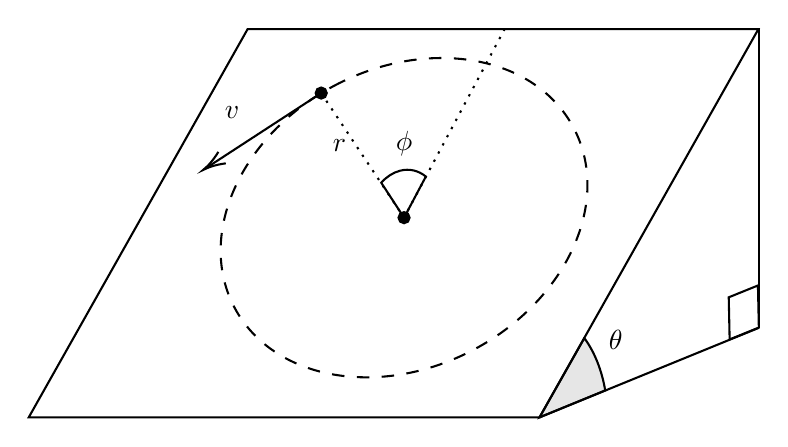
\begin{tikzpicture}[x=0.75pt,y=0.75pt,yscale=-1,xscale=1]
%uncomment if require: \path (0,300); %set diagram left start at 0, and has height of 300

%Straight Lines [id:da47922463191494025] 
\draw    (404.77,80.73) -- (404.77,224.73) ;
%Shape: Pie [id:dp6052033696960859] 
\draw  [color={rgb, 255:red, 0; green, 0; blue, 0 }  ,draw opacity=1 ][fill={rgb, 255:red, 216; green, 216; blue, 216 }  ,fill opacity=0.64 ] (320.7,229.78) .. controls (325.52,236.35) and (329.08,245.08) .. (330.76,255.01) -- (299.09,268) -- cycle ;
%Shape: Parallelogram [id:dp3636291479456979] 
\draw   (158.47,80.92) -- (404.56,80.92) -- (299.09,268) -- (53,268) -- cycle ;
%Straight Lines [id:da07860560767008584] 
\draw    (404.56,224.92) -- (299.09,268) ;
%Shape: Ellipse [id:dp33809398213922104] 
\draw  [dash pattern={on 4.5pt off 4.5pt}] (200.07,108.27) .. controls (245.16,84.3) and (296.83,93.29) .. (315.47,128.36) .. controls (334.12,163.43) and (312.68,211.29) .. (267.6,235.26) .. controls (222.51,259.24) and (170.84,250.24) .. (152.2,215.18) .. controls (133.55,180.11) and (154.99,132.25) .. (200.07,108.27) -- cycle ;
%Shape: Circle [id:dp9660949777850081] 
\draw  [fill={rgb, 255:red, 0; green, 0; blue, 0 }  ,fill opacity=1 ] (191.25,111.74) .. controls (191.25,110.26) and (192.45,109.06) .. (193.92,109.06) .. controls (195.4,109.06) and (196.6,110.26) .. (196.6,111.74) .. controls (196.6,113.21) and (195.4,114.41) .. (193.92,114.41) .. controls (192.45,114.41) and (191.25,113.21) .. (191.25,111.74) -- cycle ;
%Straight Lines [id:da054710075011608295] 
\draw    (193.92,111.74) -- (138.68,147.71) ;
\draw [shift={(137,148.8)}, rotate = 326.93] [color={rgb, 255:red, 0; green, 0; blue, 0 }  ][line width=0.75]    (10.93,-3.29) .. controls (6.95,-1.4) and (3.31,-0.3) .. (0,0) .. controls (3.31,0.3) and (6.95,1.4) .. (10.93,3.29)   ;
%Shape: Circle [id:dp16939027997095324] 
\draw  [fill={rgb, 255:red, 0; green, 0; blue, 0 }  ,fill opacity=1 ] (231.16,171.77) .. controls (231.16,170.29) and (232.36,169.09) .. (233.84,169.09) .. controls (235.31,169.09) and (236.51,170.29) .. (236.51,171.77) .. controls (236.51,173.25) and (235.31,174.44) .. (233.84,174.44) .. controls (232.36,174.44) and (231.16,173.25) .. (231.16,171.77) -- cycle ;
%Straight Lines [id:da20455724854353496] 
\draw  [dash pattern={on 0.84pt off 2.51pt}]  (193.92,111.74) -- (233.84,171.77) ;
%Shape: Parallelogram [id:dp8445337594196616] 
\draw   (404.77,224.73) -- (404.34,204.44) -- (390.27,210.14) -- (390.7,230.43) -- cycle ;
%Straight Lines [id:da05309378649652152] 
\draw  [dash pattern={on 0.84pt off 2.51pt}]  (282.35,80.77) -- (233.84,171.77) ;
%Shape: Pie [id:dp8762145687246736] 
\draw  [color={rgb, 255:red, 0; green, 0; blue, 0 }  ,draw opacity=1 ] (222.85,154.93) .. controls (225.38,152.09) and (228.47,150.03) .. (231.89,149.15) .. controls (236.49,147.96) and (240.87,149.11) .. (244.34,151.96) -- (233.84,171.77) -- cycle ;

% Text Node
\draw (331,224.4) node [anchor=north west][inner sep=0.75pt]    {$\theta $};
% Text Node
\draw (198,132.8) node [anchor=north west][inner sep=0.75pt]    {$r$};
% Text Node
\draw (146,116.6) node [anchor=north west][inner sep=0.75pt]    {$v$};
% Text Node
\draw (228.4,128.8) node [anchor=north west][inner sep=0.75pt]    {$\phi $};


\end{tikzpicture}   